\section{Method}
\label{sec:method}

This is method. And the figure \ref{fig:banana} shows the banana.

\begin{figure}
    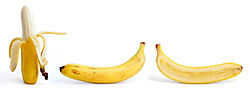
\includegraphics[width=\textwidth]{figures/banana.jpg}
    \caption{Banana}
    \label{fig:banana}
\end{figure}

% COMMENTING OUT THE NOTES
% - select sample of urban areas (FUA)
% - fetch the data from OSM
% - polygonize the network
% - measure shape charactersitics
%     - TODO: measure initally more than Reock (get a sample from ESDA)
%     - there is a conceptual backbone to this - we know that the artifacts are either
%     small (small intersections) polygons or can be large but then they are very narrow
%     (in between dual carriegaway)
%     - we need a shape metric that captures this relationship
% - identify optimal measurements
%     - plots that help us visually detect a cluster of artifacts
% - derivation of 1-dimensional index
%     - from Roeck and area we can derive one value from which distribution we can
%     identify a cut-off value for artifact/non-artifact polygons
% - cut-off value detection
% - exploration of geographical variation
%     - differences between cities and continents
% - open tools, open data, open code with full reproducibility

% METHOD SECTION ON FINDING THE MINIMUM AND USING IT AS THRESHOLD. SOME OF IT SHOULD GO IN RESULTS MAYBE?
Many, though not all, shape index frequency distributions for the analyzed FUAs reveal a common feature of two prominent peaks (see figure [INSERT FIG REF]). Through visual analysis, we find that these peaks represent two different types of polygons. Most of the polygons from the first (leftmost) peak can be attributed to ``bananas’’ in the street network, whereas most of the polygons from the second (rightmost) peak represent true urban blocks. Therefore, for FUAs that show a pronounced two-peak pattern in their shape index frequency distribution, the minimum \textit{between} the two peaks can be used as shape index threshold: polygons with a shape index below the threshold will most likely be ``bananas’’; polygons with a shape index above the threshold will most likely be true urban blocks. To derive the minimum, we approximate the shape index frequency distribution with a Gaussian kernel density estimation. For bandwidth selection, we use the parametric Silverman method \cite{silverman_using_1981} and find that it gives satisfactory results; non-parametric bandwidth selection methods might be a subject for future work (see section [REF]). 

Next, comparing the positions of peak 1, peak 2, and shape index threshold for different FUAs with pronounced two-peak patterns, we find that maxima positions vary to a considerably greater extent than minima positions. In other words, shape index thresholds for ``banana’’ identification from morphologically different FUAs lie within a relatively narrow range. We therefore hypothesize that applying a shape index threshold within the range identified from FUAs whose polygons follow a two-peak distribution will allow the identification of ``bananas’’ polygons even for those FUAs whose distributions do not show a two-peak pattern. Applying the … [TBD: lower boundary/median/average/higher boundary] of the empirically derived shape index threshold range to the rest of FUAs indeed reveals ``bananas´´ polygons in all/most FUAs (see Figure [REF]).
